%!TEX encoding = UTF-8 Unicode
%!TEX TS-program = xelatex

%%%%%%%%%%%%%%%%%%%%%%%%%%%%%%%%%%%%%%%%%
%
% Connor Johnson
% CMPT 435L_111_23S
% Spring 2023
% Lab0/ Git/LaTeX
%
%%%%%%%%%%%%%%%%%%%%%%%%%%%%%%%%%%%%%%%%%


%----------------------------------------------------------------------------------------
%	PACKAGES AND OTHER DOCUMENT CONFIGURATIONS
%----------------------------------------------------------------------------------------



\documentclass[a4paper,12pt]{article}
\usepackage[margin=22mm]{geometry}
\usepackage{fontspec,xltxtra,polyglossia,titling,graphicx}
\usepackage{verbatim,gb4e,synttree,multicol} % choose or add what you need
\usepackage[colorlinks,urlcolor=blue,citecolor=blue,linkcolor=blue]{hyperref}
\setmainfont[Mapping=tex-text]{Times New Roman} % or another similar font
\setdefaultlanguage{english}
\setotherlanguages{norsk}
\usepackage{natbib}
\bibliographystyle{apalike}
\frenchspacing
\newcommand{\tig}[1] {\fontspec{Abyssinica SIL} #1} 
\usepackage{graphicx}
\graphicspath{ {./images/} }

\title{Assignment 0: Git and LaTeX} 
\author{Connor H. Johnson \\ connor.johnson1@marist.edu}
\hyphenation{lem-mat-iz-at-ion uni-code}

\begin{document}
\begin{center} \vfill
\textbf{\Large Marist College}

{\large MS in Computer Science

School of Computer Science and Mathematics \vfill

CMPT-435L-111-23s Algorithm Analysis and Design 

Brian Gormanly

Spring 2023 

\vfill

\includegraphics[width=0.5\textwidth]{Marist.png} \vfill

\emph{\Large\thetitle} \vfill 
\theauthor} \vfill

\end{center} \clearpage
\maketitle

\begin{center}
\begin{large}
    Overview
\end{large}    
\end{center}

\begin{center} \noindent
Within this document, I would like to go step-by-step to give you an overview of what my favorite piece of code does.
Off of personal preference, I enjoy doing a lot of front-end development. Seeing what I produce brings me back to languages like HTML, EJS, CSS, and many more. I find that running my websites off of localhost and using Nodemon is the easiest way to produce my work quickly and for me not to go through continuous tedious steps to host my website. 
This document will show the mandatory code and package installations to host a localhost web page using Nodemon properly for files in EJS and CSS.
\end{center}

\begin{center}
    -----------------------------------------------------------------------
\end{center}

\begin{center}
\begin{large}
    Step-by-Step Instructions
\end{large}
\end{center}


To begin, you will need to start a new file inside your code editor. My favorite is Visual Studio Code (VSCode), as I find the environment very clean and easy to comprehend, unlike other editors.
\begin{footnotesize}
For more information about VSCode, I recommend visiting their website\footnote{Visual Studio Code: \url{https://code.visualstudio.com/}} 
\end{footnotesize}

\section{Installation of the Packages:}

Once you obtain a blank document inside VSCode, we will open a new terminal.

To open the terminal:

\begin{itemize}
  \item Use the \verb| Windows: Ctrl+, Linux: Ctrl+` | keyboard shortcut to toggle the terminal panel.
  \item Use the \verb| Windows: Ctrl+Shift+, Linux: Ctrl+Shift+` | keyboard shortcut to create a new terminal.
  \item Use the \textbf{View > Terminal or Terminal > New Terminal} menu commands.
  \item From the Command Palette \verb| Windows: Ctrl+Shift+P, Linux: Ctrl+Shift+P |, use the View: Toggle Terminal command.
\end{itemize}



\pagebreak Now that the terminal is open, we are going to have to use the \verb|'npm'| command to install our packages into our project. Once the code provided below is executed into the terminal, we now have installed a \verb|node_modeules|, \verb|package-lock.json|, and a \verb|package.json| file so that our website can host properly.

Package installation commands:
\begin{enumerate}
  \item \verb|npm init -y|
  \item \verb|npm i express ejs|
  \item \verb|npm i -D nodemon|
\end{enumerate}

\section{Edit the Package}

Although we installed these packages, there are still some changes we will have do for them to work properly.

Below is what your \verb|package.json| file should look like:
\begin{verbatim}
    {
      "name": "johnsonwebsite",
      "version": "1.0.0",
      "description": "My personal website -- soon to be hosted -- currently ran by local host",
      “main”: "index.js",
      "scripts": {
        "scripts":{"start":"echo \ "Error: no test specified:\""&& exit 1 "    
    },
      },
      "repository": {
        "type": "git",
        "url": "git+https://github.com/connorjohnson6/JohnsonWebsite.git"
      },
      "keywords": [],
      "author": "",
      "license": "ISC",
      "bugs": {
        "url": "https://github.com/connorjohnson6/JohnsonWebsite/issues"
      },
      "homepage": "https://github.com/connorjohnson6/JohnsonWebsite#readme",
      "dependencies": {
        "ejs": "^3.1.8",
        "express": "^4.18.2",
        "express-ejs-layouts": "^2.5.1"
      },
      "devDependencies": {
        "nodemon": "^2.0.20"
      }
    }
\end{verbatim}
\pagebreak However, we will change the \verb|"main"|(line 5) and add some functions to our \verb|"scripts"|(Line 7). We are doing this mainly to communicate with our soon-to-be-created \verb|app.js| file and to add some shortcuts to properly call our Nodemon package in our terminal for our web page to run when no errors occur continuously.

Below is what your \verb|package.json| file should look now look like when edited:
\begin{verbatim}
    {
      "name": "johnsonwebsite",
      "version": "1.0.0",
      "description": "My personal website -- soon to be hosted -- currently ran by local host",
      "main": "app.js",
      "scripts": {
        "start": "node app.js",
        "dev": "nodemon app.js"
      },}}
      "repository": {
        "type": "git",
        "url": "git+https://github.com/connorjohnson6/JohnsonWebsite.git"
      },
      "keywords": [],
      "author": "",
      "license": "ISC",
      "bugs": {
        "url": "https://github.com/connorjohnson6/JohnsonWebsite/issues"
      },
      "homepage": "https://github.com/connorjohnson6/JohnsonWebsite#readme",
      "dependencies": {
        "ejs": "^3.1.8",
        "express": "^4.18.2",
        "express-ejs-layouts": "^2.5.1"
      },
      "devDependencies": {
        "nodemon": "^2.0.20"
      }
    }
\end{verbatim}

\pagebreak\section{Add your folders and files}

Now that we properly have everything downloaded, we will make a file named \verb|app.js|(\ref{ex:dutch}) and two folders named \textbf{views}(\ref{ex:tigrinya}) and \textbf{public}(\ref{ex:app}).
 
\begin{exe}
\ex \label{ex:dutch}
\gll App.js\\

\begin{large} \textbf{App.js}\end{large} \\
\begin{itemize}
\item The code below is mandatory as this is how you implement the Express and EJS packages. Line 1-3 allows you to use express while the next line assigns a port number you want to run your LocalHost from. Many choose their port number to be, for example, 3000, 4000, or 5000. 
\item Following that are the static files that allow your soon-to-be-created EJS files to connect to each other and allow you to use CSS and JavaScript and upload images.
\item In your next section of code, you're to set up your engine. On line 14, you can see that we have our views folder named in the \textbf{app.set} as this is what we will call from due to it soon holding our EJS files.
\item The rest of your code will be your navigation within your search bar. These six lines of code are what you will put into your navbar when your host your website. For example, \verb|Localhost:3000/about| will bring you to your \textbf{about page} later created in your views folder. Following that is an \verb|app.listen| command that will communicate with express to host your page via your desired port. 
\end{itemize}
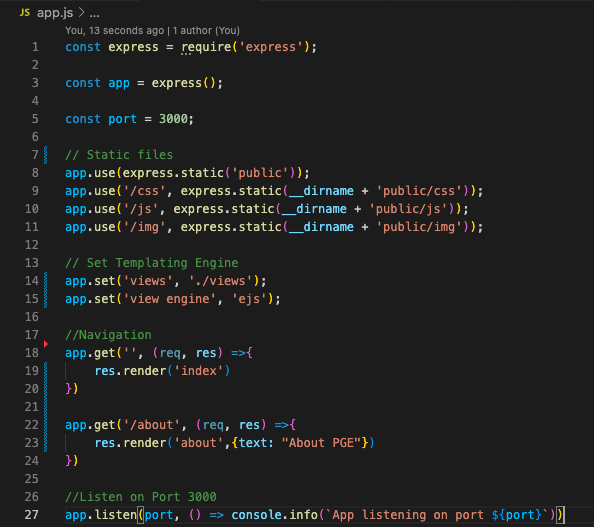
\includegraphics[scale=.7]{appjs.png} 
\end{exe}


\begin{exe}
\ex \label{ex:tigrinya}
\glll Views\\

\begin{large} \pagebreak\textbf{Views}\end{large} \\
\begin{itemize}
\item Now that we have our express working and hosting a live port using Nodemon, we can customize our views folder. Inside of here will be our HTML, or in this case, EJS files. We will be creating two EJS files, \textbf{index.ejs} and \textbf{about.ejs}. Just so nothing gets complicated, inside our index.ejs and about.ejs, we can insert a \verb|!| tag and press enter to insert the needed parameters automatically. \\

The HTML code will look like this:
\begin{verbatim}
<!DOCTYPE html>
<html lang="en">
<head>
    <meta charset="UTF-8">
    <meta http-equiv="X-UA-Compatible" content="IE=edge">
    <meta name="viewport" content="width=device-width, initial-scale=1.0">
    <title>Document</title>
</head>
<body>
    
</body>
</html>
\end{verbatim}

Once this is done, we must link our CSS page inside our index.ejs file. In addition, we will also add a title to our page and a \verb|<h1>Hello World<\h1>| so that we know that the website is working.\\

The HTML code will now look like this:
\begin{verbatim}
<!DOCTYPE html>
<html lang="en">
<head>
    <meta charset="UTF-8">
    <meta http-equiv="X-UA-Compatible" content="IE=edge">
    <meta name="viewport" content="width=device-width, initial-scale=1.0">
    <link rel="stylesheet" href="/style.css">
    <title>Index</title>
</head>
<body>

    <h1>Hello World</h1>

</body>
</html>
\end{verbatim}


\end{itemize}
\end{exe}


\begin{exe}
\ex \label{ex:app}
\gll Public\\ 

\begin{large} \pagebreak\textbf{Public}\end{large}
\begin{itemize}
\item Now that we have already planned for a CSS page inside of our index.ejs page, we now must add a file called \verb|style.css| inside of our public folder
\item since a CSS folder will be filled with your own code to customize, for now, we are just going to make the background blue just so we can see if the CSS is correctly implemented inside of our index.ejs page.\\

The CSS code we will include is:
\begin{verbatim}
body{
    background-color: blue
}
\end{verbatim}
\end{itemize}
 
\end{exe}


\section{Live hosting your website}
Now that we have everything properly set up, we will now host our website on a browser using a local host\\
Inside our terminal in VSCode, we will now write and enter:
\begin{itemize}
    \item \verb|npm run dev|
\end{itemize}

\begin{center}
When we enter \verb|localhost:3000| in the browser of your choice, the result should be:
\end{center}

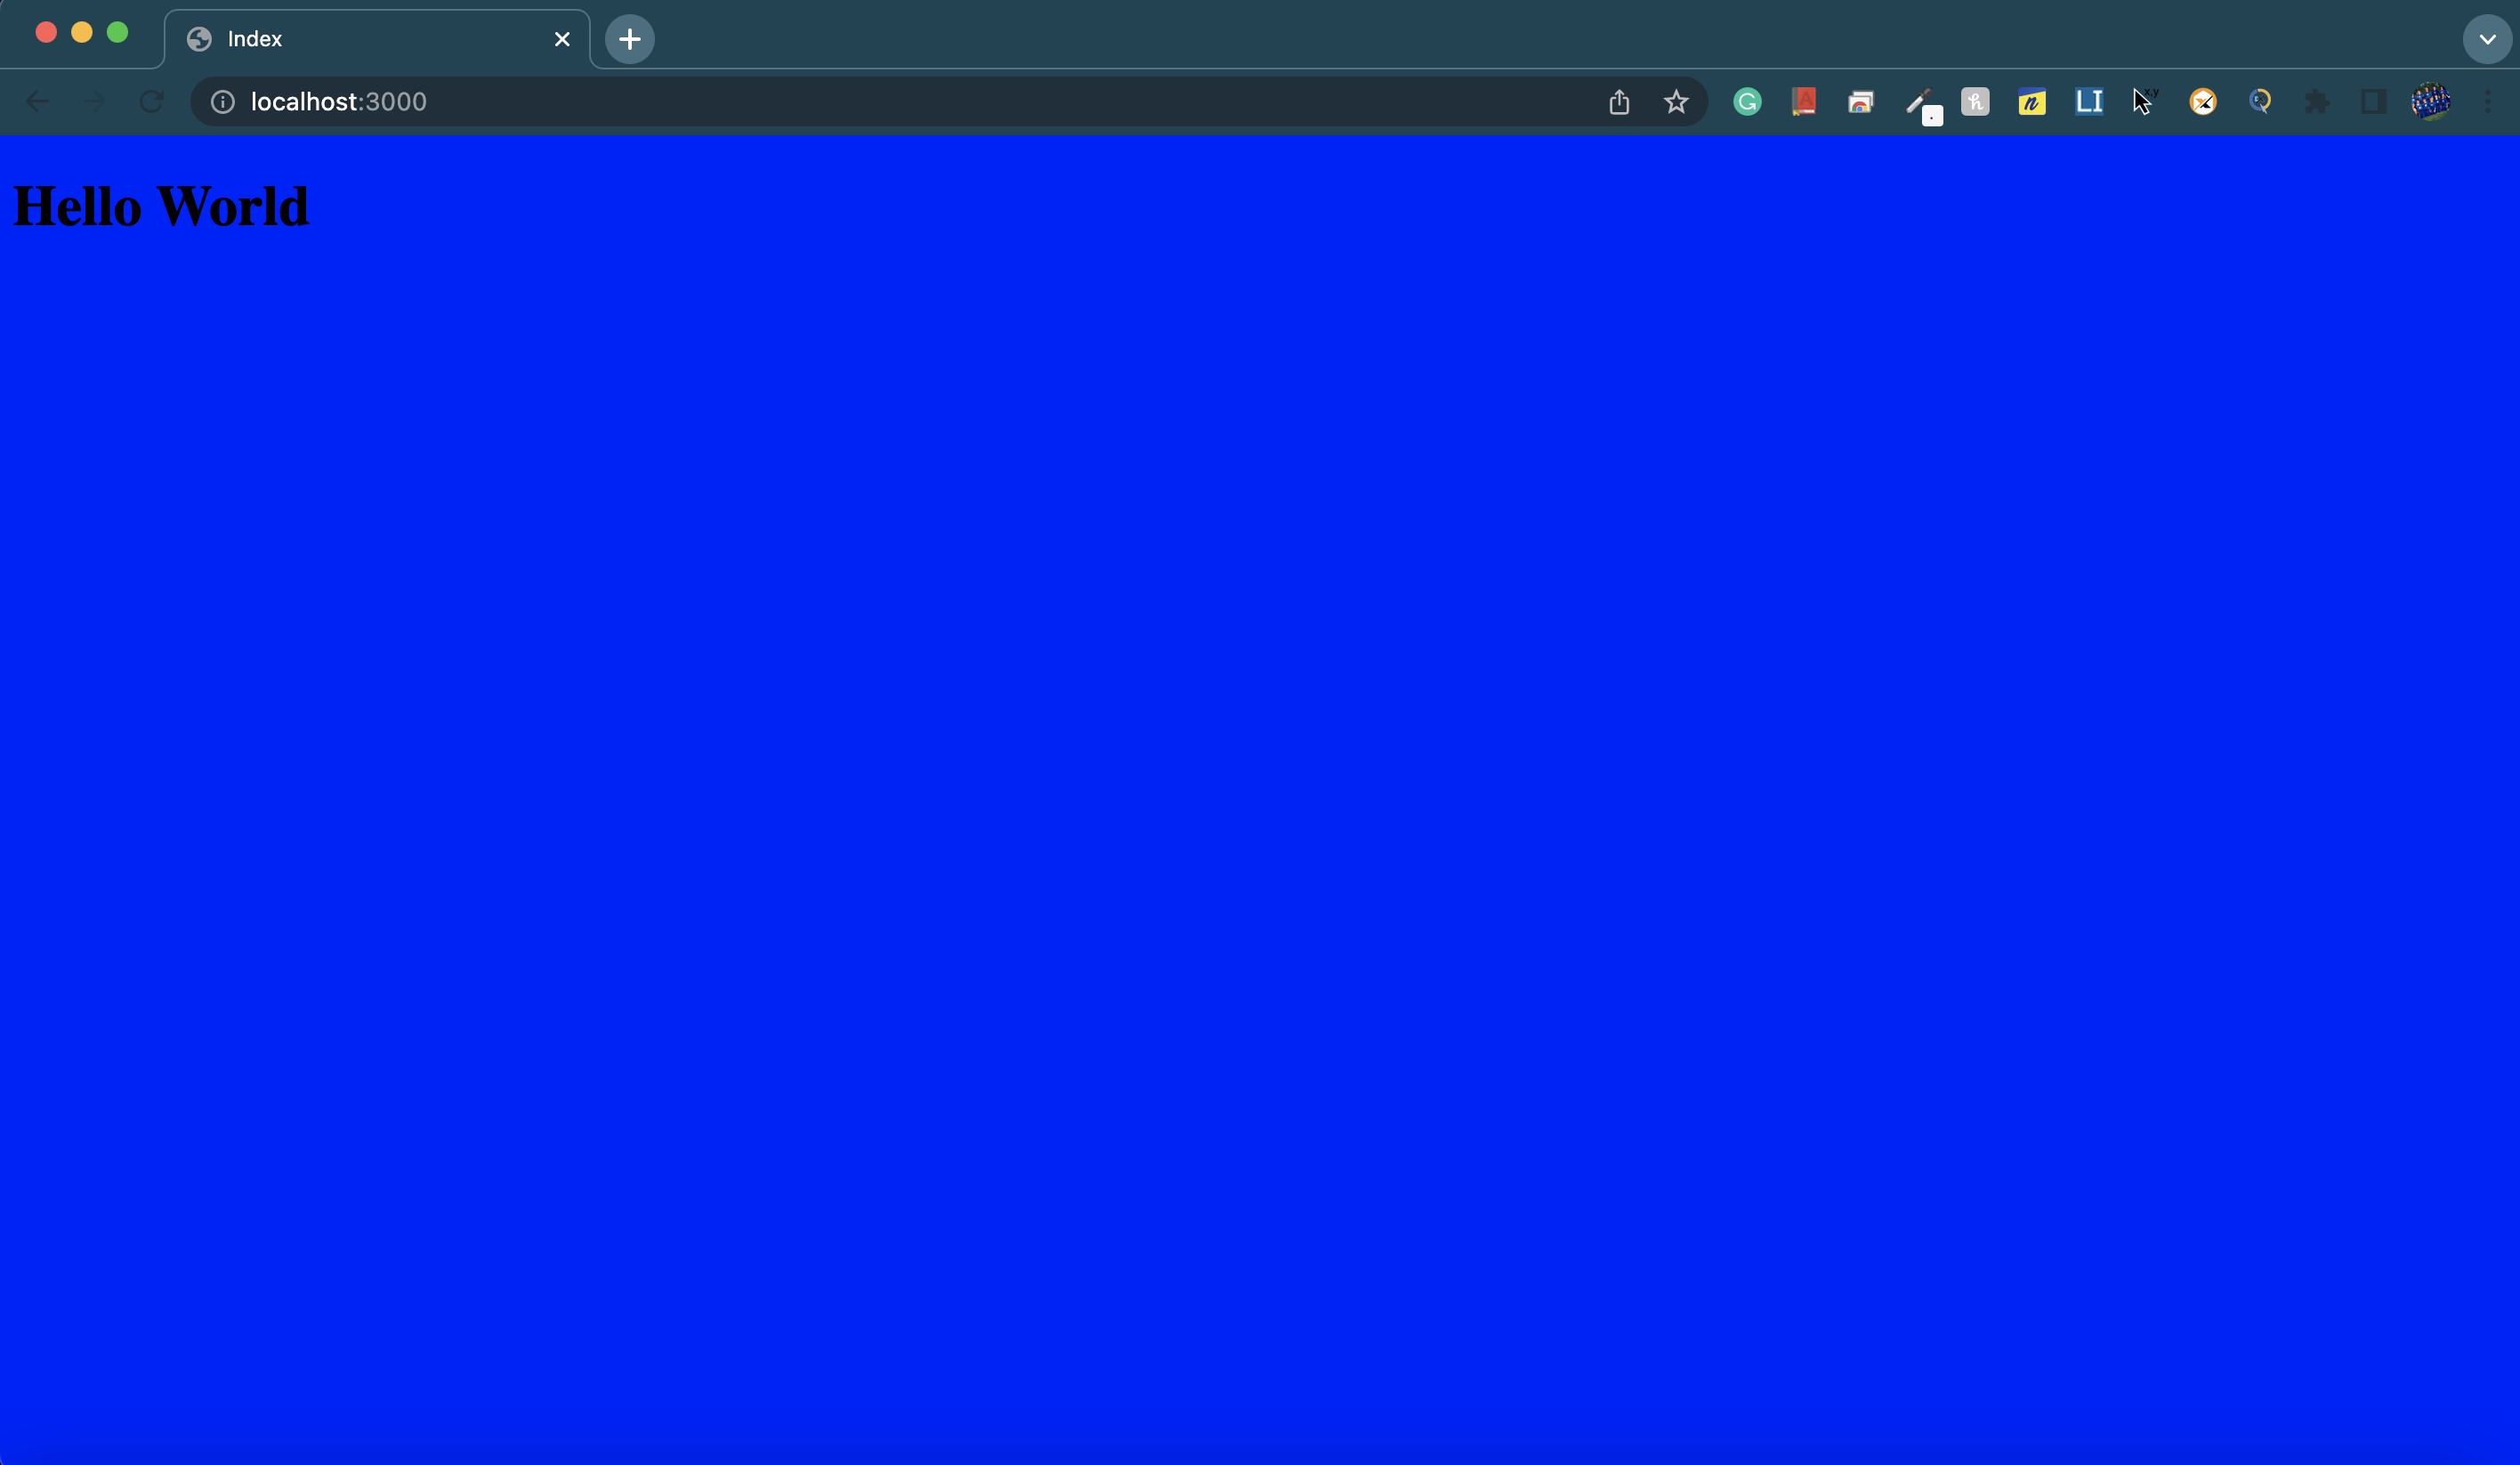
\includegraphics[scale=.3]{localhost.png} 


\section{Customization}

Now that you have successfully hosted a server and connected your EJS and CSS files, you can now start customizing your website to your liking! 

\end{document}
